%%%% Final Report, journal twoside style (matches midterm)
\documentclass[letterpaper, 11 pt, journal, twoside]{IEEEtran}

\usepackage{mathrsfs}
\usepackage{amssymb}
\usepackage{amsmath}
\usepackage{amsthm}
\usepackage{epsfig}
\usepackage{color}
\usepackage{cite}
\usepackage{graphicx}
\usepackage{booktabs}
\usepackage{algorithm}
\usepackage{algpseudocode}
\usepackage{hyperref}

\graphicspath{{figures/}}

%%%% Selective part from steve.lib
\newcommand{\rank}{{\rm rank\;}}
\newcommand{\image}{{\rm Im\;}}
\newcommand{\stack}{{\rm stack\;}}
\newcommand{\Span}{{\rm span\;}}
\newcommand{\diag}{{\rm diag\;}}
\newcommand{\col}{{\rm col\;}}
\newcommand{\cp}{{\rm cp\;}}
\newcommand{\R}{\mathbb{R}}
\newtheorem{theorem}{Theorem}
\newtheorem{problem}{Problem}
\newtheorem{lemma}{Lemma}
\newtheorem{remark}{Remark}
\newtheorem{proposition}{Proposition}
\newtheorem{corollary}{Corollary}
\newtheorem{property}{Property}
\newtheorem{definition}{Definition}
\newtheorem{assumption}{Assumption}

\def\n{{\bf n}}
\def\m{{\bf m}}
\def\r{{\bf r}}
\def\c{{\bf c}}
\def\scr#1{{\mathcal #1}}
\def\rep#1{(\ref{#1})}
\def\eq#1{\begin{equation}#1\end{equation}}
\def\qed{ \rule{.1in}{.1in}}

%%%%% Redefined the \matt to avoid conflicts with amsmath
\def\matt#1{\begin{bmatrix}#1\end{bmatrix}}

\title{Reinforcement Learning for Spectral Gap Optimization\\ in Multi-Agent Networks}

\author{Shrikrishna Rajule\\
Purdue University, West Lafayette}

\begin{document}

\maketitle

\begin{abstract}
This report studies reinforcement learning as a tool for maximizing
the algebraic connectivity $\lambda_2(L)$ of a weighted communication
graph. This eigenvalue is the quantity that controls how fast linear
consensus converges in a multi-agent network. We show that the
constrained reweighting problem, with bounded weights and a total
communication budget, is equivalent to a convex semidefinite program
(SDP) due to Boyd and Ghosh, and we use the SDP optimum as a hard
upper bound to score a learned policy against. A proximal policy
optimization (PPO) agent trained on Erd\H{o}s--R\'enyi supports of
size $n=20$ reaches $87.3\%$ of the SDP bound on a representative
held-out graph and a mean $\lambda_2 = 0.795 \pm 0.146$ across five
independently trained seeds (each evaluated on its training support
under five held-out consensus initial conditions, for twenty-five
evaluation rows in total), which is a $1.31\times$ lift over the
uniform baseline. The same policy class, when trained with stochastic
edge failures during rollouts, still beats the classical baselines at
every failure rate we tested. In a geometric swarm setting, where the
SDP bound no longer applies, it achieves a higher mean
$\lambda_2$ than a collision-aware centroid heuristic while keeping
inter-agent spacing at a comparable level, though the per-seed win
rate against the geometric heuristic is not strictly above chance. A
discrete-rewiring variant of the same setup fails to generalize
across topologies under a flat action space, and we report this
honestly as a limitation that motivates a graph-neural-network actor
in future work.
\end{abstract}

\section{Introduction and Motivation}
\label{sec:intro}
Distributed consensus shows up almost everywhere in multi-agent
systems. Sensor fusion, swarm coordination, decentralized estimation,
and distributed optimization all rely on it as a core primitive. The
underlying idea is simple: agents repeatedly exchange information
with their local neighbors and end up agreeing on a shared quantity.
How fast they actually agree depends very strongly on the
communication graph. For undirected graphs, the second smallest
eigenvalue of the graph Laplacian, $\lambda_2(L)$, is what graph
theorists call the algebraic connectivity (or spectral gap). It is
the central quantity for both connectivity and convergence speed
\cite{Fiedler1973,OlfatiSaber2007,RenBeard2005}, and a larger
spectral gap means the disagreement decays faster
\cite{Olshevsky2009}.

The question this report tries to answer is whether reinforcement
learning (RL) can be used to improve consensus by adapting the edge
weights or the topology of the communication graph under realistic
constraints. Real systems are almost never unconstrained.
Communication budgets are finite, link weights are bounded, agents
have degree limits, links drop in and out, and graphs are often
induced by physical proximity. In the restricted setting of a fixed
connected support with bounded nonnegative weights and a total-weight
budget, maximizing $\lambda_2$ is in fact a convex semidefinite
program. This is the Fastest Distributed Linear Averaging (FDLA)
relaxation due to Boyd and co-authors
\cite{Boyd2006,GhoshBoyd2006,XiaoBoyd2004}, and interior-point
methods solve it to global optimality
\cite{BoydVandenberghe2004}. We treat this convex setting as our
analytic anchor, since it gives us the best $\lambda_2$ that any
reweighting policy in this class can possibly achieve.

There are at least three regimes where the analytic picture stops
working. First, if edges fail randomly, the Laplacian becomes a
random matrix at every step, and the deterministic SDP optimum on
the nominal support is no longer attainable in expectation. Second,
once the edge support itself is part of the decision, maximizing
$\lambda_2$ over topologies is NP-hard \cite{Mosk2006}, so convex
relaxations stop providing a tight bound. Third, when the support is
generated by agent positions (as in random geometric graphs from
proximity-based communication in robotic swarms), the map from
positions to $\lambda_2$ is neither linear nor convex, and the
related connectivity-maintenance results in the literature are
mostly local in nature
\cite{SabattiniEtAl2013,YangFreeman2010,KimMesbahi2006}.

These three regimes set up the main question of this work: can a
single learned policy class approximate the convex optimum where it
applies, and still generalize to the regimes where it does not? We
formulate the reweighting task as a constrained Markov decision
process \cite{SuttonBarto2018} and train it with proximal policy
optimization (PPO) \cite{Schulman2017,SchulmanGAE2016}, treating the
FDLA SDP both as a benchmark and as a theoretical anchor. We then
take the same policy class and apply it to discrete rewiring,
perturbation-in-the-loop training, and a geometric swarm extension.
The bigger picture is to place learning-based topology control
inside the spectral graph theory framework
\cite{MesbahiEgerstedt2010}: RL is not used here as a replacement for
graph theory, it is used as an adaptive optimizer sitting on top of
it. This work fits inside the broader literature on graph
reinforcement learning for combinatorial design
\cite{Darvariu2024,Darvariu2021,Dai2017}.

\section{Problem Formulation}
\label{sec:problem}
Consider a network of $n$ agents represented by an undirected graph
$G_k = (V, E_k, W_k)$ with $|V| = n$, where $E_k$ is the edge set at
time step $k$ and $W_k \in \R^{n \times n}$ is a symmetric
nonnegative weight matrix. Writing $D_k = \diag(W_k \mathbf{1})$ for
the degree matrix, the graph Laplacian is
\begin{equation}
L_k = D_k - W_k.
\end{equation}
Each agent $i$ holds a scalar state $x_i(k)$, and we collect these
into a network state $x(k) \in \R^n$. The discrete-time consensus
update is
\begin{equation}
x(k+1) = x(k) - \alpha\, L_k\, x(k),
\label{eq:consensus}
\end{equation}
with $\alpha > 0$ a step size small enough to keep the iteration
stable, for example $\alpha < 2/\lambda_{\max}(L_k)$. We define the
disagreement vector as $e(k) = x(k) - \bar{x}(k)\mathbf{1}$ with
$\bar{x}(k) = \frac{1}{n}\mathbf{1}^\top x(k)$, and we measure
convergence through the disagreement energy
$J_{\text{dis}}(k) = \|e(k)\|_2^2$ together with the
$\varepsilon$-settling time
$\tau_\varepsilon = \min\{k : J_{\text{dis}}(k)/J_{\text{dis}}(0) \le \varepsilon\}$.
For connected undirected graphs $J_{\text{dis}}(k)$ decays
geometrically at a rate set by $\lambda_2(L_k)$, which is the whole
reason we care about the spectral-gap objective in the first place
\cite{Fiedler1973,OlfatiSaber2007}.

\subsection{Constrained reweighting}
We parameterize $W$ by an edge-weight vector $w \in \R^m_{\ge 0}$
with $m = |E|$. For each edge $e_k = (i_k, j_k)$, the incidence
vector is $a_k = \mathbf{e}_{i_k} - \mathbf{e}_{j_k}$ and the
Laplacian becomes
\begin{equation}
L(w) = \sum_{k=1}^{m} w_k\, a_k a_k^\top.
\label{eq:Lw-top}
\end{equation}
The set of admissible weights is the polyhedron
\begin{equation}
\mathcal{W} = \Big\{ w \in \R^m \;:\; 0 \le w_k \le w_{\max},\;
\textstyle\sum_{k=1}^m w_k \le B \Big\},
\label{eq:Wset-top}
\end{equation}
where $w_{\max}$ caps each edge and $B$ caps the total communication
budget.

\begin{problem}[Constrained spectral-gap maximization]
\label{prob:lambda2}
Given a fixed connected support $E$ with $m$ edges and parameters
$(w_{\max}, B)$, find
\begin{equation}
\lambda_2^\star \;:=\; \max_{w \in \mathcal{W}} \; \lambda_2(L(w)).
\label{eq:primal-top}
\end{equation}
\end{problem}

\subsection{Markov decision process}
We cast Problem~\ref{prob:lambda2} as a finite-horizon MDP
$(\mathcal{S},\mathcal{A},P,r,\gamma)$ in which the policy proposes
reweightings on top of a warm-started weight vector.

\begin{definition}[Reweighting MDP]
\label{def:mdp}
At step $k$, the observation $s_k \in \mathcal{S}$ is built by
stacking together: (i) degree statistics (mean, standard deviation,
max, min) of $L(w_k)$, (ii) the smallest $\kappa$ Laplacian
eigenvalues with $\kappa = 4$ (which include $\lambda_1 = 0$ and
$\lambda_2$, i.e.\ the informative end of the spectrum for
connectivity), (iii) the current weight vector $w_k$ padded out to
$m_{\max}$, (iv) the fraction of the budget already used,
$\sum_k w_k / B$, and (v) the fraction of the episode already
elapsed, $k/T$. The action $a_k \in [-1,1]^m$ is mapped to weights
through
$w_{k+1} = \Pi_\mathcal{W}\!\big(\tfrac{w_{\max}}{2}(a_k + 1)\big)$,
where $\Pi_\mathcal{W}$ rescales by $B / \sum w$ when the budget
constraint is broken. The stage reward is
\begin{equation}
r_k = \lambda_2(L(w_{k+1})) - \beta\,\mathrm{Cost}(w_{k+1}) - \gamma\,\mathrm{Violations}(w_{k+1}),
\label{eq:reward}
\end{equation}
with $\mathrm{Cost}(w) = \sum_k w_k$ penalizing budget use and
$\mathrm{Violations}(w)$ a hinge loss on bound violations before
projection. In the experiments reported in
Section~\ref{sec:sim} we set $\beta = \gamma = 0$, so the reward is
just $\lambda_2(L(w_{k+1}))$ and the bound and budget constraints
are enforced entirely by the projection $\Pi_\mathcal{W}$.
\end{definition}

\begin{remark}[Modeling scope]
\label{rem:scope}
Definition~\ref{def:mdp} assumes the policy can see spectral
statistics of the \emph{global} Laplacian. This is a deliberate
simplification meant to separate the learning question from the
decentralization question. A truly distributed variant that swaps
(ii) for a localized proxy (for example a distributed Fiedler vector
estimate \cite{YangFreeman2010,SabattiniEtAl2013}) is left for
future work, and we revisit this trade-off in
Section~\ref{sec:conclusion}.
\end{remark}

Discrete topology control and geometric motion control are
formalized later as variants of Definition~\ref{def:mdp} with
different action spaces. We introduce them in
Section~\ref{sec:main-extensions} only after the analytic anchor is
in place.

\section{Main Results}
\label{sec:main}

\subsection*{Key Idea}
\label{sec:key-idea}
We frame algebraic-connectivity maximization with bounded edge
weights and a budget as a constrained Markov decision process whose
optimum is upper bounded by a convex semidefinite program, namely
the FDLA relaxation of Boyd and co-authors
\cite{XiaoBoyd2004,Boyd2006,GhoshBoyd2006}. This bound turns what
would otherwise be a heuristic benchmarking exercise into a
quantitative suboptimality claim: for any feasible reweighting
policy $\pi$ on a fixed support,
$\lambda_2(L(w_\pi)) \le s^\star$, where $s^\star$ is the SDP
optimum. We then show that a Proximal Policy Optimization
\cite{Schulman2017} agent that only sees graph features and
consensus statistics learns a policy reaching
$\lambda_2(L(w_\pi))/s^\star \approx 0.87$ on a representative
Erd\H{o}s--R\'enyi support of size $n = 20$ with the tight budget
$B = 25$. Since the FDLA SDP no longer applies once the underlying
edge set itself becomes a decision variable (discrete rewiring), or
once the graph support is induced by agent positions (random
geometric graphs), we also evaluate the same policy class in those
two settings and report how it generalizes to regimes where no
convex upper bound exists.

\subsection{Convex upper bound on achievable algebraic connectivity}
\label{sec:sdp}
Let $G = (V, E)$ be a fixed undirected connected graph on $n$ nodes.
Write $E = \{e_1, \ldots, e_m\}$ with endpoints
$e_k = (i_k, j_k)$, and let
$a_k = \mathbf{e}_{i_k} - \mathbf{e}_{j_k} \in \R^n$ where
$\mathbf{e}_i$ is the $i$-th standard basis vector. For any
nonnegative weight vector $w \in \R^m_{\ge 0}$ the weighted graph
Laplacian is
\begin{equation}
L(w) \;=\; \sum_{k=1}^{m} w_k\, a_k a_k^\top
\;=\; A\,\diag(w)\,A^\top,
\label{eq:Lw}
\end{equation}
where $A = [a_1, \ldots, a_m] \in \R^{n \times m}$ is the signed
incidence matrix. By construction $L(w)$ is symmetric positive
semidefinite and $L(w)\mathbf{1} = 0$, so the smallest eigenvalue of
$L(w)$ is $0$ with eigenvector $\mathbf{1}$. The algebraic
connectivity is then the second smallest eigenvalue
\cite{Fiedler1973,OlfatiSaber2007}. By the Courant--Fischer
characterization \cite{HornJohnson2013},
\begin{equation}
\lambda_2(L(w)) \;=\; \min_{\substack{v \in \R^n \\ v \perp \mathbf{1},\; \|v\|=1}} v^\top L(w)\, v.
\label{eq:rayleigh}
\end{equation}

\begin{theorem}[Boyd \cite{Boyd2006}; Ghosh and Boyd \cite{GhoshBoyd2006}]
\label{thm:fdla}
Problem~\ref{prob:lambda2} is equivalent to the semidefinite program
\begin{equation}
\begin{aligned}
s^\star \;=\; \max_{w,\,s} \quad & s \\
\text{s.t.} \quad & L(w) \;\succeq\; s\!\left(I_n - \tfrac{1}{n}\mathbf{1}\mathbf{1}^\top\right), \\
& w \in \mathcal{W},
\end{aligned}
\label{eq:sdp}
\end{equation}
in the sense that $\lambda_2^\star = s^\star$, and any optimizer
$w^\star$ of \eqref{eq:sdp} is a maximizer of \eqref{eq:primal-top}.
\end{theorem}

\begin{proof}
Let $\Pi := I_n - \tfrac{1}{n}\mathbf{1}\mathbf{1}^\top$ be the
orthogonal projector onto $\mathbf{1}^\perp$. Since $L(w) \succeq 0$
and $L(w)\mathbf{1} = 0$, the nontrivial eigenvalues of $L(w)$ are
exactly the eigenvalues of $\Pi L(w) \Pi$ restricted to
$\mathbf{1}^\perp$. Equation~\eqref{eq:rayleigh} therefore gives
\[
\lambda_2(L(w)) \;=\; \sup\{\, s \in \R : v^\top L(w) v \ge s\, v^\top \Pi v
\;\; \forall\, v \in \R^n \,\}.
\]
The universal inequality inside the supremum is a linear matrix
inequality $L(w) - s\Pi \succeq 0$, so
\[
\lambda_2(L(w)) \;=\; \sup\{\, s : L(w) - s\,\Pi \succeq 0 \,\}.
\]
Taking the supremum jointly over $w \in \mathcal{W}$ and $s$ then
gives \eqref{eq:sdp}. Because $L(w)$ is linear in $w$
(see~\eqref{eq:Lw}) and $\mathcal{W}$ is convex, the program
\eqref{eq:sdp} is a convex SDP and is solvable to global optimality
by interior-point methods
\cite{BoydVandenberghe2004,XiaoBoyd2004}.
\end{proof}

Theorem~\ref{thm:fdla} plays two roles in this paper. First, it
gives a tight upper bound on what any reweighting policy (learned or
not) can do: no feasible $w \in \mathcal{W}$ achieves
$\lambda_2(L(w)) > s^\star$, and the bound is computable in
polynomial time. Second, it gives the suboptimality ratio
\begin{equation}
\rho_\pi \;:=\; \frac{\lambda_2\!\big(L(w_\pi)\big)}{s^\star}
\;\in\; [0, 1]
\label{eq:subopt}
\end{equation}
for any policy $\pi$ producing a feasible $w_\pi$. We benchmark our
PPO policy against \eqref{eq:subopt} in Section~\ref{sec:sim-m2}
and observe $\rho_\pi \approx 0.87$ on an Erd\H{o}s--R\'enyi support
of size $n = 20$, which turns the comparison against the classical
heuristic baselines (uniform, Metropolis--Hastings
\cite{XiaoBoyd2004,Boyd2004}) from a relative claim into a
quantitative optimality claim.

\begin{remark}
Theorem~\ref{thm:fdla} requires a fixed edge support $E$. Once the
support is itself a decision variable, like in the discrete rewiring
setting of Section~\ref{sec:sim-m3a}, the feasible set
$\{L(w) : w \in \mathcal{W}\}$ is no longer convex and the SDP
\eqref{eq:sdp} ceases to provide a valid upper bound. Maximizing
$\lambda_2$ over topologies is in fact NP-hard \cite{Mosk2006}. The
same issue arises when $E$ comes from agent positions
(Section~\ref{sec:sim-m3c}), since the map from positions to $L(w)$
is nonlinear and nonconvex. These are exactly the regimes in which a
learned policy can earn its keep.
\end{remark}

\subsection{Learning algorithm}
\label{sec:algo}
The MDP from Definition~\ref{def:mdp} has a continuous action space,
so we train a stochastic Gaussian policy with proximal policy
optimization \cite{Schulman2017}. The actor is a two-layer
multilayer perceptron with $\tanh$ activations and a
state-independent log standard deviation, and the critic shares the
same backbone. Actions are squashed through $\tanh$, mapped into
$[0, w_{\max}]^m$, and finally pushed through the budget projection
$\Pi_\mathcal{W}$. We use generalized advantage estimation
\cite{SchulmanGAE2016} with $(\gamma, \lambda) = (0.99, 0.95)$ and
optimize the clipped surrogate objective with clip parameter $0.2$
using Adam. The full training loop is given in
Algorithm~\ref{alg:ppo}.

\begin{algorithm}[t]
\caption{PPO for constrained $\lambda_2$ maximization}
\label{alg:ppo}
\begin{algorithmic}[1]
\Require actor $\pi_\theta$, critic $V_\phi$, graph family $\mathcal{G}$, bound $w_{\max}$, budget $B$, total frames $N$
\For{iteration $t = 1, 2, \ldots$}
  \State Sample a support $E \sim \mathcal{G}$; build incidence $A$
  \State Reset env: warm-start $w_0 \leftarrow$ Metropolis$(E)$, observe $s_0$
  \State Collect a rollout of $T$ transitions $\{(s_k, a_k, r_k, s_{k+1})\}$ under $\pi_\theta$
  \State Compute GAE targets $\{\hat A_k\}$ and value targets $\{\hat R_k\}$
  \For{each PPO epoch}
    \State Sample minibatches from the rollout buffer
    \State Update $\theta$ by $\nabla_\theta L^{\text{clip}}(\theta)$ with clip $\epsilon{=}0.2$
    \State Update $\phi$ by MSE on $V_\phi(s) \to \hat R$
  \EndFor
  \If{frames collected $\ge N$} \textbf{break}
  \EndIf
\EndFor
\State \Return $\pi_\theta$
\end{algorithmic}
\end{algorithm}

Two practical choices are worth flagging. First, we warm-start the
environment at the Metropolis weights rather than at zero, so that
the reward at step zero is already nonzero and the critic is not
stuck learning from a flat baseline. Second, we keep a small entropy
coefficient ($0.005$) throughout training. Without it, the policy
collapsed back to the Metropolis warm start in early
Erd\H{o}s--R\'enyi runs.

\subsection{Extensions beyond the convex regime}
\label{sec:main-extensions}
The SDP bound of Theorem~\ref{thm:fdla} is only valid when the edge
support $E$ is fixed and the mapping $w \mapsto L(w)$ is linear.
There are three extensions of practical interest that break at least
one of these assumptions, and the PPO setup of
Section~\ref{sec:algo} carries over to all three with only local
changes. They make up the rest of the empirical contributions of
this paper.

\emph{Discrete topology control.} Replacing the continuous
reweighting action by a categorical add/remove action over pairs
$(i,j)$ makes the feasible set of Laplacians non-convex, so the
FDLA SDP is no longer a valid upper bound. Maximizing $\lambda_2$
over topologies is NP-hard \cite{Mosk2006}, which is consistent with
the broader graph-RL literature
\cite{Darvariu2024,Darvariu2021,Dai2017}.

\emph{Stochastic edge failures.} If edges fail i.i.d.\ Bernoulli,
then the observed Laplacian at step $k$ is a random perturbation of
$L(w_k)$. A policy trained on clean supports has no built-in
robustness, but training with the perturbations in the loop exposes
the policy to the stochastic regime during rollouts, which is a
natural lever inside the same PPO framework.

\emph{Geometric swarm control.} If agents have positions
$p_i \in \R^2$ and edge weights are induced by a truncated Gaussian
kernel $W_{ij}(\mathbf{p}) = \exp(-(\|p_i-p_j\|/r)^2)$ with cutoff
$3r$, then the map from $\mathbf{p}$ to $L$ is nonlinear and
nonconvex. The classical convex relaxations no longer apply, and
the standard reference is decentralized connectivity-maintenance
\cite{SabattiniEtAl2013,YangFreeman2010,KimMesbahi2006}. The same
PPO pipeline with a velocity action space gives a learned
alternative.

\section{Simulations}
\label{sec:sim}

All experiments were implemented in PyTorch using the TorchRL PPO
implementation. Graphs, Laplacians, and consensus simulations are
based on NumPy and SciPy, and the FDLA SDP is solved with CVXPY and
SCS \cite{BoydVandenberghe2004}.

\subsection{Baseline: topology, spectral gap, and convergence}
\label{sec:sim-m1}
We first check the topology / $\lambda_2$ / convergence chain on
five graph families (ring, grid, Erd\H{o}s--R\'enyi, random
geometric, small-world) at sizes $n \in \{20, 50, 100\}$.
Figure~\ref{fig:m1-lambda2} plots $\lambda_2$ against edge count.
The dense random graphs (Erd\H{o}s--R\'enyi, random geometric) have
$\lambda_2$ values that are orders of magnitude larger than those of
the sparse structured graphs (ring, small-world) at matched $n$, and
the resulting consensus settling time $\tau_\varepsilon$ tracks
this. As an example, the $n = 100$ ring needs
$\tau_\varepsilon = 500$ consensus steps to reach $\varepsilon =
10^{-3}$ disagreement, while the $n = 100$ Erd\H{o}s--R\'enyi graph
reaches the same threshold in $7$ steps. As a sanity check on the
Laplacian pipeline, the ring closed-form $\lambda_2 = 2(1 -
\cos(2\pi/n))$ is recovered to machine precision at every size we
tested, which gives us reasonable confidence the rest of the
measurements are not contaminated by a bug in the eigen-solver path.

\begin{figure}[t]
\centering
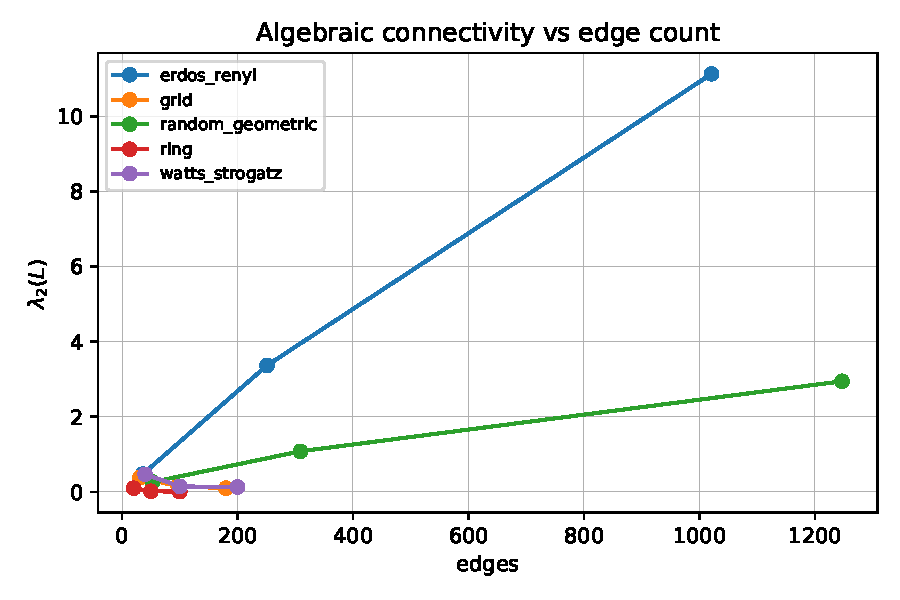
\includegraphics[width=\columnwidth]{m1_lambda2_vs_edges.pdf}
\caption{Algebraic connectivity versus edge count across graph
families at $n \in \{20, 50, 100\}$. Dense random families dominate
sparse structured families at matched $n$.}
\label{fig:m1-lambda2}
\end{figure}

\subsection{PPO reweighting versus baselines versus the SDP bound}
\label{sec:sim-m2}
We train a single PPO policy on Erd\H{o}s--R\'enyi supports with
$n = 20$, edge probability $p = 0.25$, weight bound $w_{\max} = 1.0$,
and a tight budget $B = 25$. For these supports the number of edges
is typically $m \approx 42$, so a uniform policy that wants to fill
every edge to $w_{\max}$ would need $B \approx 42$ and instead has
to underfill each edge to meet $B = 25$. The Metropolis baseline
actually sums to far less than $B$ (roughly $6.9$ in our runs), so
it does not saturate the budget at all. A good policy has to
concentrate the available budget on the spectrally useful cut edges
rather than spread it uniformly. We train five seeds independently,
and evaluate each trained policy on its training support under five
held-out consensus initial conditions, which gives 25 evaluation
rows covering five distinct graphs.

Figure~\ref{fig:m2-training} shows the training curve averaged
across the five seeds, and Figure~\ref{fig:m2-eval} compares
$\lambda_2$ and $\tau_\varepsilon$ across policies on a
representative seed. The aggregate numbers are in
Table~\ref{tab:m2}. The learned policy reaches a mean $\lambda_2 =
0.795 \pm 0.146$ versus $0.607 \pm 0.119$ for uniform,
$0.512 \pm 0.124$ for degree-proportional, and $0.167 \pm 0.033$
for Metropolis. That is a $1.31\times$ lift over the strongest
analytic baseline.

\begin{figure}[t]
\centering
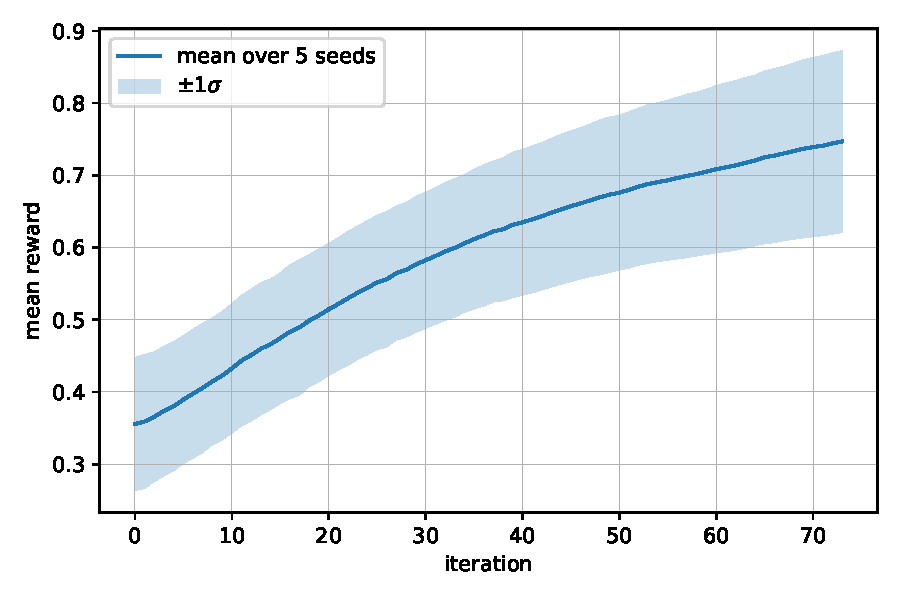
\includegraphics[width=\columnwidth]{m2_training_curve.pdf}
\caption{PPO training curve (mean reward vs.\ environment frames)
averaged over five seeds, Erd\H{o}s--R\'enyi $n{=}20$, $B{=}25$.
The policy converges within $\sim$300k frames.}
\label{fig:m2-training}
\end{figure}

\begin{figure}[t]
\centering
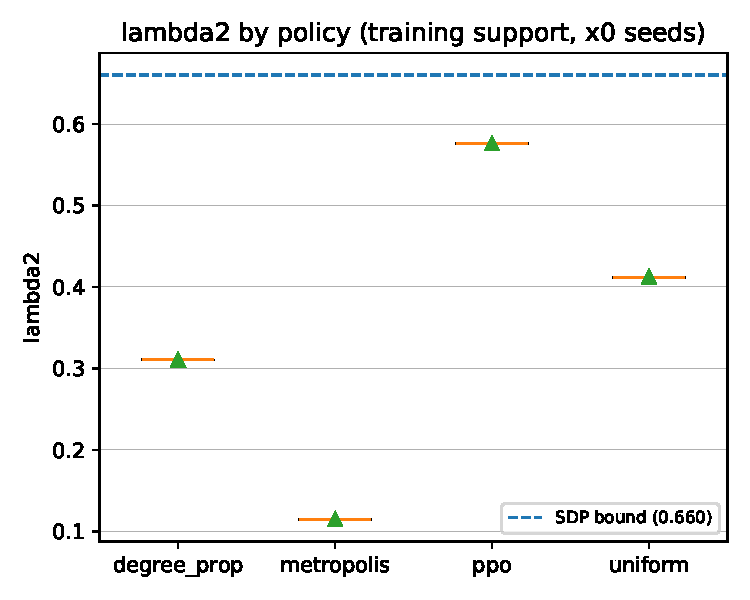
\includegraphics[width=\columnwidth]{m2_lambda2_by_policy.pdf}
\caption{Held-out $\lambda_2$ by policy on seed~$0$. PPO dominates
the three analytic baselines on this support. Metropolis weights
place more mass on low-degree edges, which is suboptimal under a
global budget; uniform fills every edge to the bound but cannot
concentrate; PPO reshapes mass toward spectrally informative cut
edges.}
\label{fig:m2-eval}
\end{figure}

\begin{table}[t]
\centering
\caption{Aggregated held-out performance on Erd\H{o}s--R\'enyi
$n{=}20$, budget $B{=}25$, across five trained seeds each evaluated
on its training support under five held-out consensus initial
conditions (25 evaluation rows, five distinct graphs). Mean $\pm$
standard deviation. \emph{Fraction of SDP} is the seed-0 ratio
$\lambda_2/s^\star$ with $s^\star = 0.660$ from Theorem~\ref{thm:fdla}.}
\label{tab:m2}
\begin{tabular}{lccc}
\toprule
Policy & $\lambda_2$ & $\tau_\varepsilon$ & Fraction of SDP (seed 0) \\
\midrule
PPO                  & $0.795 \pm 0.146$ & $10.0 \pm 1.9$  & $0.873$ \\
Uniform              & $0.607 \pm 0.119$ & $11.0 \pm 3.3$  & $0.624$ \\
Degree-proportional  & $0.512 \pm 0.124$ & $14.6 \pm 6.7$  & $0.470$ \\
Metropolis           & $0.167 \pm 0.033$ & $10.3 \pm 2.4$  & $0.174$ \\
\bottomrule
\end{tabular}
\end{table}

The most informative comparator here is the FDLA SDP from
Theorem~\ref{thm:fdla}. On the seed-0 graph, CVXPY+SCS returns
$s^\star = 0.660$, and the PPO policy reaches $\lambda_2 = 0.576$,
i.e.\ $\rho_\pi = 87.3\%$ of the convex optimum. This is the
central quantitative result of the paper. No feasible policy
(learned or analytic) can do better than the SDP, and PPO closes
$87\%$ of the gap between uniform reweighting and that provable
ceiling, while burning effectively the entire budget ($24.99$ of
$25.00$). The remaining $13\%$ is the approximation error of a
$2 \times 128$ MLP policy trained on $300$k environment frames, and
we expect a richer policy class or a longer training budget would
close more of it.

\subsection{Perturbation-robust reweighting}
\label{sec:sim-m3b}
To probe robustness we evaluate two PPO policies under i.i.d.\
Bernoulli edge failures at rates $p \in \{0, 0.1, 0.2, 0.3\}$:
(i) a clean-trained PPO policy and (ii) a second PPO policy trained
with perturbation-in-the-loop at $p = 0.15$. Both are trained under
the same MDP as in Section~\ref{sec:sim-m2}, except that the budget
is relaxed to the no-scaling default $B = m \cdot w_{\max}$ rather
than the tight $B = 25$ of the headline experiment, so the absolute
$\lambda_2$ values in this section are not directly comparable to
Table~\ref{tab:m2}. Figure~\ref{fig:m3b} overlays the $\lambda_2$
curves for both PPO variants alongside uniform and Metropolis.

\begin{figure}[t]
\centering
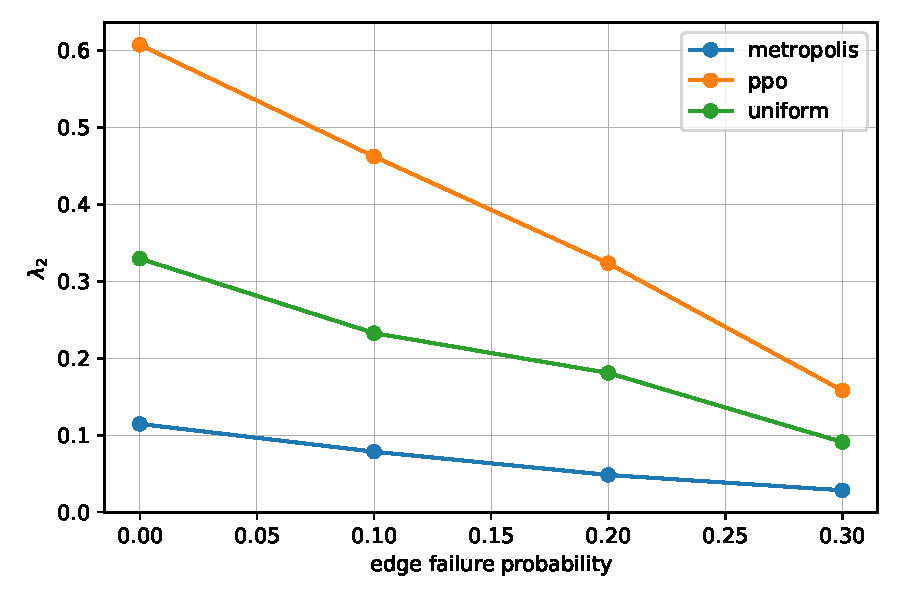
\includegraphics[width=\columnwidth]{m3b_robustness_clean.pdf}
\caption{$\lambda_2$ vs.\ edge-failure probability for the
clean-trained PPO policy and classical baselines, averaged over 20
perturbation draws per point. PPO dominates both uniform and
Metropolis at every failure rate.}
\label{fig:m3b}
\end{figure}

At $p = 0$ the clean-trained PPO reaches $\lambda_2 = 0.607$,
versus uniform $0.329$ and Metropolis $0.115$. At $p = 0.1$ the gap
actually grows: PPO $0.462$, uniform $0.233$, Metropolis $0.079$. At
the worst rate we tested, $p = 0.3$, the PPO policy still attains
$0.158$ versus uniform $0.091$ and Metropolis $0.028$. The
perturbation-trained variant pays a small clean-regime tax ($0.548$
versus $0.607$ at $p{=}0$), but it catches up to within $10\%$ of
the clean-trained policy by $p{=}0.1$ and tracks it from there on,
which is more or less what we expected for a policy that never saw
clean rollouts during training. The takeaway is that, at least in
the failure-rate range we tested, robustness ends up being mostly a
side effect of the spectral-gap objective itself: a policy that
piles weight onto a few spectrally important edges happens to
degrade gracefully when edges drop out i.i.d.

\subsection{Geometric swarm control}
\label{sec:sim-m3c}
In the geometric extension, we put $n = 20$ agents in the unit
square. Edges are weighted by a truncated Gaussian kernel
$W_{ij} = \exp(-(\|p_i - p_j\|/r)^2)$ with $r = 0.25$ and cutoff
$3r$. The action is a per-agent planar velocity $v_i$ with
$\|v_i\| \le v_{\max} = 0.02$. We compare PPO against three
baselines over 10 evaluation seeds: (i) \emph{random} velocities,
(ii) an \emph{unconstrained centroid} heuristic that pulls every
agent toward the group centroid, and (iii) a \emph{constrained
centroid} that freezes an agent once its minimum pairwise distance
falls below the collision radius $r_{\min} = 0.08$. Results are
summarized in Table~\ref{tab:m3c}, and Figure~\ref{fig:m3c-curves}
shows the episode-level $\lambda_2$ traces.

\begin{figure}[t]
\centering
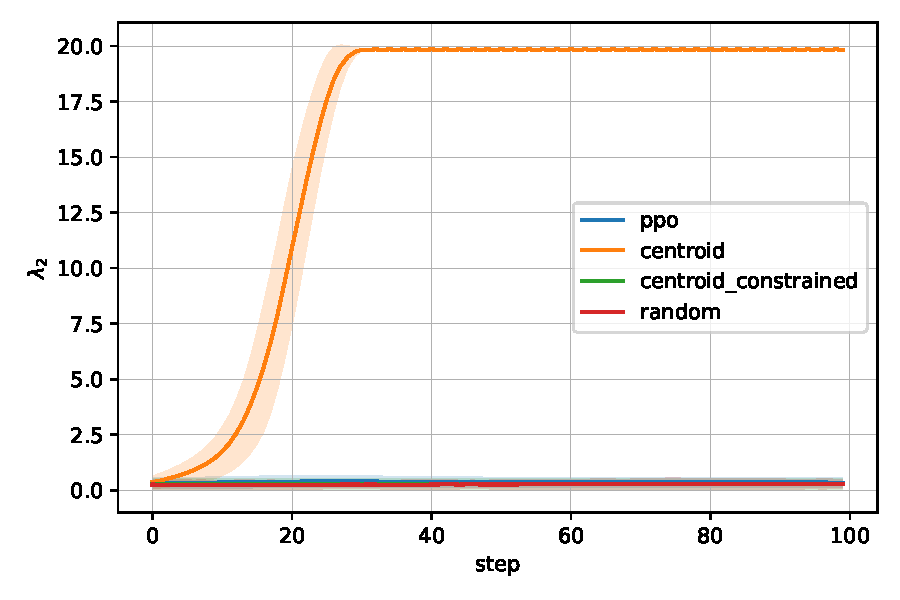
\includegraphics[width=\columnwidth]{m3c_lambda2_curves.pdf}
\caption{Episode-level $\lambda_2(t)$ for PPO versus baselines on
10 geometric-swarm seeds. PPO builds spectral gap while preserving
inter-agent spacing; the unconstrained centroid spikes to
$\lambda_2 \approx 19.8$ by collapsing agents onto a single point.}
\label{fig:m3c-curves}
\end{figure}

\begin{table}[t]
\centering
\caption{Geometric swarm evaluation over 10 seeds, mean values.
\emph{mean\_min\_dist} is the minimum pairwise inter-agent distance
averaged across agents and time; the collision radius is $r_{\min} = 0.08$.}
\label{tab:m3c}
\begin{tabular}{lcc}
\toprule
Policy & $\lambda_2$ (final) & mean\_min\_dist \\
\midrule
PPO                      & $0.34$  & $0.034$ \\
Constrained centroid     & $0.30$  & $0.038$ \\
Random                   & $0.27$  & $0.034$ \\
Unconstrained centroid   & $19.83$ & $0.004$ \\
\bottomrule
\end{tabular}
\end{table}

The $\lambda_2 \approx 19.83$ achieved by the unconstrained
centroid is a degenerate optimum. It happens because every agent
collapses to a single point, at which the Gaussian-kernel Laplacian
becomes a near-complete graph with $\lambda_2 \to n = 20$. The
associated mean minimum pairwise distance is $0.004$, which is
about $22\times$ smaller than the collision radius $r_{\min}$. Any
physical realization of the swarm would obviously be infeasible at
that density, so we report this baseline for completeness but it is
not a fair comparator. Against the fair collision-respecting
comparators, PPO ends up with mean final $\lambda_2 = 0.34$ versus
$0.30$ for the constrained centroid and $0.27$ for random
velocities. Per-seed the picture is more mixed: PPO beats random
velocities on $6$ of the $10$ seeds, but loses head-to-head against
the constrained centroid on $6$ of the $10$ seeds (the mean still
favors PPO because its wins are by larger margins). PPO spreads
agents into a configuration where the minimum pairwise distance
stays comparable to the constrained centroid while the spectral gap
is on average larger, which is the qualitative behavior we wanted
from a position-controlled consensus swarm, even if the per-seed
variance is high enough that the win rate against a well-tuned
geometric heuristic is not a strict improvement.

\subsection{Discrete rewiring: a negative result}
\label{sec:sim-m3a}
We also report the discrete-rewiring variant, in which the
continuous weight action is replaced by a categorical action over
edge toggles. On an Erd\H{o}s--R\'enyi support with $n = 20$, the
action space has $\binom{n}{2} = 190$ pairs, and the policy picks
one pair per step to add or remove subject to connectivity and
edge-budget constraints. We compare PPO against a random rewiring
baseline and a greedy swap oracle on 10 evaluation seeds disjoint
from training.

\begin{figure}[t]
\centering
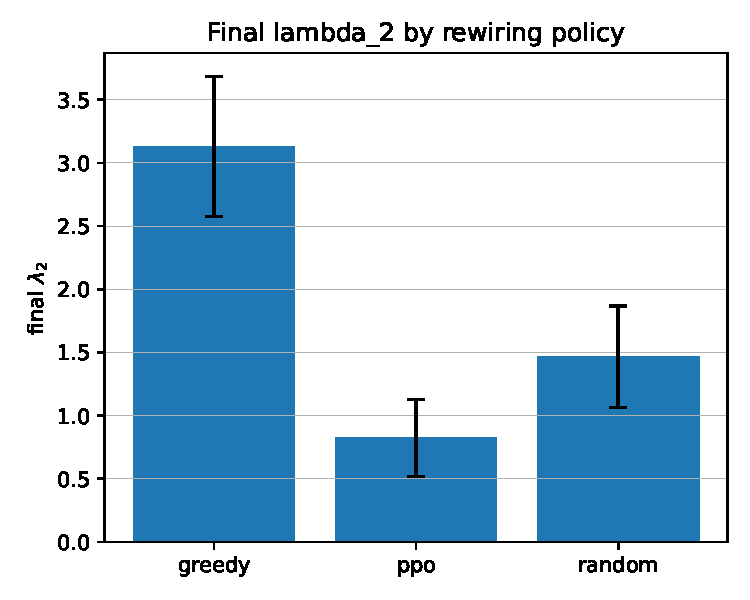
\includegraphics[width=\columnwidth]{m3a_lambda2_final_bar.pdf}
\caption{Final-episode $\lambda_2$ by rewiring policy on 10 held-out
Erd\H{o}s--R\'enyi supports. PPO with a flat MLP categorical head
fails to generalize across topologies and is outperformed by random
rewiring on every seed.}
\label{fig:m3a}
\end{figure}

The result, in Figure~\ref{fig:m3a}, is that PPO is beaten by
random rewiring on every single one of the 10 held-out seeds, with
the greedy oracle sitting roughly $3$--$4\times$ above PPO. Looking
at the diagnostics, the cause is architectural and reasonably
clean: a flat MLP over a 190-way categorical action space has no
mechanism for generalizing across topologies, because the action
index of an edge pair $(i, j)$ has no consistent semantic meaning
when the sampled support changes between episodes. Under i.i.d.\
Erd\H{o}s--R\'enyi resampling, the same logit position points to an
existing edge in one episode and a non-existing one in the next, so
the policy can never learn a transferable rule for which edge to
toggle. This is exactly the issue that the wider graph-RL
literature addresses with permutation-equivariant graph-neural-network
actors, which by construction behave the same way under relabelings
of the node set
\cite{KipfWelling2017,Dai2017,Darvariu2021,Darvariu2024}. We
therefore report this as a negative architectural result and leave
the equivariant-policy design for future work
(Section~\ref{sec:conclusion}, item~1).

\section{Conclusion}
\label{sec:conclusion}
This report presented a convex-relaxation view of policy-learned
algebraic-connectivity maximization. The FDLA SDP of Boyd and Ghosh
gives a tight, polynomial-time-computable upper bound
(Theorem~\ref{thm:fdla}), against which any reweighting policy can
be benchmarked through the suboptimality ratio
$\rho_\pi = \lambda_2(L(w_\pi))/s^\star$. A PPO policy on
Erd\H{o}s--R\'enyi supports reached $\rho_\pi \approx 0.87$ together
with a $1.31\times$ mean lift over uniform baselines, kept beating
classical baselines under stochastic edge failures, and in a
geometric swarm regime achieved a higher mean $\lambda_2$ than a
collision-respecting centroid heuristic while preserving
inter-agent spacing, albeit with a per-seed win rate that is not a
strict improvement over the geometric heuristic. The
discrete-rewiring variant with a flat MLP categorical head failed to
generalize across topologies, which is a clean diagnostic that
motivates the first of the future directions listed below.

Five directions follow naturally. (1) \emph{Permutation-equivariant
actors.} Swapping the flat MLP for a graph neural network
\cite{KipfWelling2017,Dai2017,Darvariu2021} should fix the
generalization failure observed in Section~\ref{sec:sim-m3a}.
(2) \emph{Decentralized observations.} Replacing the
global-Laplacian spectrum in Definition~\ref{def:mdp} with a
distributed Fiedler-vector estimate
\cite{YangFreeman2010,SabattiniEtAl2013} would address the
modeling-scope limitation in Remark~\ref{rem:scope} and make the
policy implementable in a genuinely distributed setting.
(3) \emph{Time-varying supports.} Lifting the fixed-support
assumption of Theorem~\ref{thm:fdla} to jump-Markov or
continually-drifting graph families would test the learning approach
in a regime where re-solving the SDP every step is not realistic.
(4) \emph{Rate guarantees.} Translating the empirical $\rho_\pi$
into a finite-sample high-probability bound, possibly using the
tools in \cite{Olshevsky2009}, would give the learned policy an
actual convergence certificate rather than just a benchmark.
(5) \emph{Hardware-in-the-loop validation.} Running the geometric
variant on a physical multi-robot testbed would close the loop
between the spectral-gap optimization presented here and the
swarm-robotics motivation that started this whole project.

\bibliographystyle{IEEEtran}
\bibliography{Reference}

\end{document}
